% `template.tex', a bare-bones example employing the AIAA class.
%
% For a more advanced example that makes use of several third-party
% LaTeX packages, see `advanced_example.tex', but please read the
% Known Problems section of the users manual first.
%
% Typical processing for PostScript (PS) output:
%
%  latex template
%  latex template   (repeat as needed to resolve references)
%
%  xdvi template    (onscreen draft display)
%  dvips template   (postscript)
%  gv template.ps   (onscreen display)
%  lpr template.ps  (hardcopy)
%
% With the above, only Encapsulated PostScript (EPS) images can be used.
%
% Typical processing for Portable Document Format (PDF) output:
%
%  pdflatex template
%  pdflatex template      (repeat as needed to resolve references)
%
%  acroread template.pdf  (onscreen display)
%
% If you have EPS figures, you will need to use the epstopdf script
% to convert them to PDF because PDF is a limmited subset of EPS.
% pdflatex accepts a variety of other image formats such as JPG, TIF,
% PNG, and so forth -- check the documentation for your version.
%
% If you do *not* specify suffixes when using the graphicx package's
% \includegraphics command, latex and pdflatex will automatically select
% the appropriate figure format from those available.  This allows you
% to produce PS and PDF output from the same LaTeX source file.
%
% To generate a large format (e.g., 11"x17") PostScript copy for editing
% purposes, use
%
%  dvips -x 1467 -O -0.65in,0.85in -t tabloid template
%
% For further details and support, read the Users Manual, aiaa.pdf.


% Try to reduce the number of latex support calls from people who
% don't read the included documentation.
%


\typeout{}\typeout{If latex fails to find aiaa-tc, read the README file!}
%


\documentclass[]{aiaa-tc}% insert '[draft]' option to show overfull boxes
\usepackage{float}
\usepackage{epstopdf}

\title{Single-Axis Control of a Solar Sail Through a Gimbal}

\author{
	Johnathan Clouse%
	\thanks{Graduate Students, Aerospace Engineering Sciences, 1111 Engineering Drive, Boulder, CO, 80309-0429}\\
	{\normalsize\itshape
		University of Colorado, Boulder, CO, 80309-0429, USA}
}

% Define commands to assure consistent treatment throughout document
\newcommand{\eqnref}[1]{(\ref{#1})}
\newcommand{\class}[1]{\texttt{#1}}
\newcommand{\package}[1]{\texttt{#1}}
\newcommand{\file}[1]{\texttt{#1}}
\newcommand{\BibTeX}{\textsc{Bib}\TeX}

\usepackage[euler]{textgreek}
\usepackage[colorlinks=true]{hyperref}
\hypersetup{urlcolor=cyan}

\usepackage{listings}
\usepackage{color} %red, green, blue, yellow, cyan, magenta, black, white
\definecolor{mygreen}{RGB}{28,172,0} % color values Red, Green, Blue
\definecolor{mylilas}{RGB}{170,55,241}

\usepackage{tablefootnote}
\usepackage{graphicx}
\usepackage{amsmath}
\usepackage{bm}
\usepackage{subfigure}
%\usepackage{subcaption}

\definecolor{mylilas}{RGB}{170,55,241}

% See p.105 of "TeX Unbound" for suggested values.
% See pp. 199-200 of Lamport's "LaTeX" book for details.
%   General parameters, for ALL pages:
\renewcommand{\topfraction}{0.9}	% max fraction of floats at top
\renewcommand{\bottomfraction}{0.8}	% max fraction of floats at bottom
%   Parameters for TEXT pages (not float pages):
\setcounter{topnumber}{2}
\setcounter{bottomnumber}{2}
\setcounter{totalnumber}{4}     % 2 may work better
\setcounter{dbltopnumber}{2}    % for 2-column pages
\renewcommand{\dbltopfraction}{0.9}	% fit big float above 2-col. text
\renewcommand{\textfraction}{0.07}	% allow minimal text w. figs
%   Parameters for FLOAT pages (not text pages):
\renewcommand{\floatpagefraction}{0.7}	% require fuller float pages
% N.B.: floatpagefraction MUST be less than topfraction !!
\renewcommand{\dblfloatpagefraction}{0.7}	% require
    \makeatletter
    \renewcommand\l@section{\@dottedtocline{2}{1.5em}{3em}}
    \makeatother
    
\begin{document}
	

	
	\maketitle
	
	\begin{abstract}
		\noindent 
		
	\end{abstract}
	
	\newpage
	
	\tableofcontents
	
	\newpage

	\section{Introduction}
Single-axis control of a solar-sail-driven interplanetary spacecraft (sailcraft) is proposed.  The attitude control system will be responsible for ensuring that the steering angle between the force and velocity vectors is within the tolerance necessary for an interplanetary voyage.  This steering angle is dependent on the mission parameters and the orbital position of the spacecraft. It, and the sun vector, will be treated as external commands to the system. The spacecraft will perform all its thrusting in the orbit plane.
	
	\vspace{5 mm}
	
The primary actuation mechanism will be a gimbaled control boom between the sail subsystem and the spacecraft bus, which contains the majority of the spacecraft mass.  With the center of mass between the thrust point and the sun, expected disturbances will cause oscillation about some angle between the sun and the axis normal to the sail, $\alpha$, for a locked gimbal.  Changing the gimbal angle, $\delta$, will dampen this oscilation with the right conrol law. Roll and pitch angles wil be held to zero for this analysis. Star trackers will determin attitude.
	
	\vspace{5 mm}

The state-space model is expected to have four states: the sun angle ($\alpha$), the rate of the sun angle ($\dot{\alpha}$), the gimbal angle ($\delta$), and the gimbal angle rate ($\dot{\delta}$).  Depending on the vane implementation, there may be up to two more states for vane angles.
	
	\vspace{5 mm}

The sail and boom will be modeled as rigid bodies, justified by the slow actuation of the gimbal throughout the flight. The sail will be modeled as a thin plate, rather than a billowed sail. Solar pressure torques (about the non-steered axis) will be controlled against. Disturbance torques from thruster firings may also be modeled. 
	
	\vspace{5 mm}

The state-space model will be obtained in a similar manner to that presented by Wie. The equations of motion for a gimbaled thrust vector are obtained for the yaw axis. 
	
	\vspace{5 mm}

System performance will be judged by the response to errors, both with a step-error and a flight-like error where the steering angle constantly-but-slowly changes. Mitigation of disturbance torques will also be examined.

	\section{State Space Representation}

	The equations of motion were linearized about the state $\alpha = \dot{\alpha} = \delta = \dot{\delta} =0$. This state is in equilibrium, due to the the force resulting from the solar radiation pressure acting through the sailcraft's center of mass.  Any disturbance to $\alpha$ would cause oscillation about $\alpha=0$. The linearized equations are shown below:

	\begin{equation}
\begin{bmatrix}
\dot{\alpha }\\ 
\ddot{\alpha}\\ 
\dot{\delta }\\ 
\ddot{\delta }
\end{bmatrix}=\begin{bmatrix}
0 & 1 & 0 & 0\\ 
0 & 0 & \frac{d}{J_s}F_n & 0\\ 
0 & 0 & 0 & 1\\ 
-\frac{m_pl}{J_pm+m_sm_pl^{2}}F_t & 0 & -\frac{m_pl}{J_pm+m_sm_pl^{2}}F_n & 0
\end{bmatrix}
\begin{bmatrix}
\alpha\\ 
\dot{\alpha}\\ 
\delta\\ 
\dot{\delta }
\end{bmatrix}
+
\begin{bmatrix}
0\\ 
-\frac{1}{J_s}\\ 
0\\ 
\frac{1}{J_p+\frac{m_sm_p}{m}l^{2}}
\end{bmatrix}T_{gimbal}
	\end{equation}
	\begin{equation}
y = \begin{bmatrix}
1 & 0 & 0 & 0
\end{bmatrix}x+\begin{bmatrix}
0
\end{bmatrix}u
	\end{equation}
	\begin{equation}
F_n=PA(1+\rho_s+\frac{2}{3}\rho_d)
	\end{equation}
	\begin{equation}
F_t=PA(1-\rho_s)
	\end{equation}
	
	\begin{table}[H]% no placement specified: defaults to here, top, bottom, page
		\begin{center}
			\caption{Sailcraft characteristics.}
			\label{t:Primary_variables}
			\begin{tabular}{|c|c|}
\hline 
Characteristic & Value  \\ \hline
$m_s$         &     40 kg\\
$m_p$         &      116 kg \\
$m$         &     156 kg \\
$J_s$   &     6000 kg$\cdot$m\textsuperscript{2} \\
$J_p$   &     20 kg$\cdot$m\textsuperscript{2} \\
$P$   &      4.563e-6 kg/m\textsuperscript{2}\\
$A_{sail}$       &     1800 m\textsuperscript{2} \\
$l$       &   2 m \\
$d$       &     1.487 m \\
$\rho_s$ &     0.8272 \\
$\rho_d$ &     -0.5949 \\
\hline
			\end{tabular}
		\end{center}
	\end{table}  

	Using the sailcraft characteristics in Table \ref{t:Primary_variables}, the eigenvalues are found to be:
	
	\vspace{5 mm}
{\centering
 $\lambda_i = \{\pm1.1200\times10^{-2}i, \pm5.9395\times10^{-4}i\}$.\par
}
	
	\vspace{5 mm}

	The complex eigenvalues with no real parts indicate that the uncontrolled, linearized system is marginally stable. It will oscillate undamped when perturbed by a small amount, but a large disturbance could excite the modes and make the output $y$ unbounded. However, as $\alpha$ and $\delta$ each approach $\pm$90$^{\circ}$, the assumption becomes invalid. Indeed, in Figure \ref{fig:Force_linearity}, one can see that a five-percent error between the non-linear and linearized sail force occurs at approximately $\pm$20$^{\circ}$.

	\vspace{5 mm}
	
	\begin{figure}[H]
		\centering
		\subfigure[Transverse force]{
			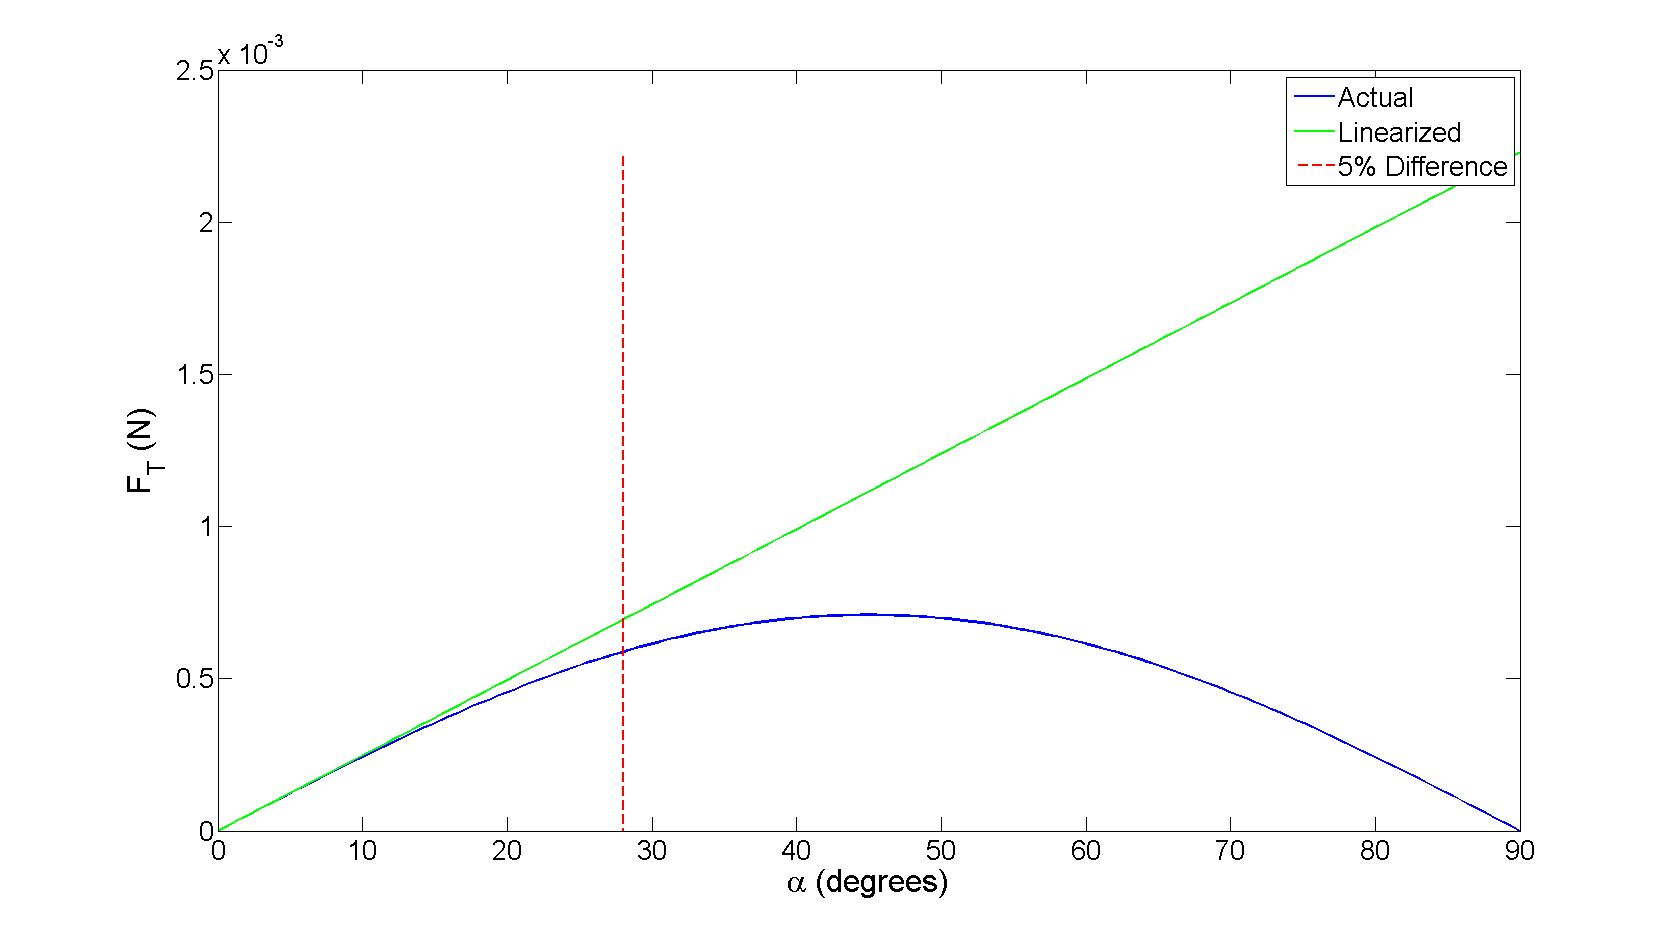
\includegraphics[width = 7.5cm]{FT_Soln.png}
		}
		\subfigure[Normal force]{
			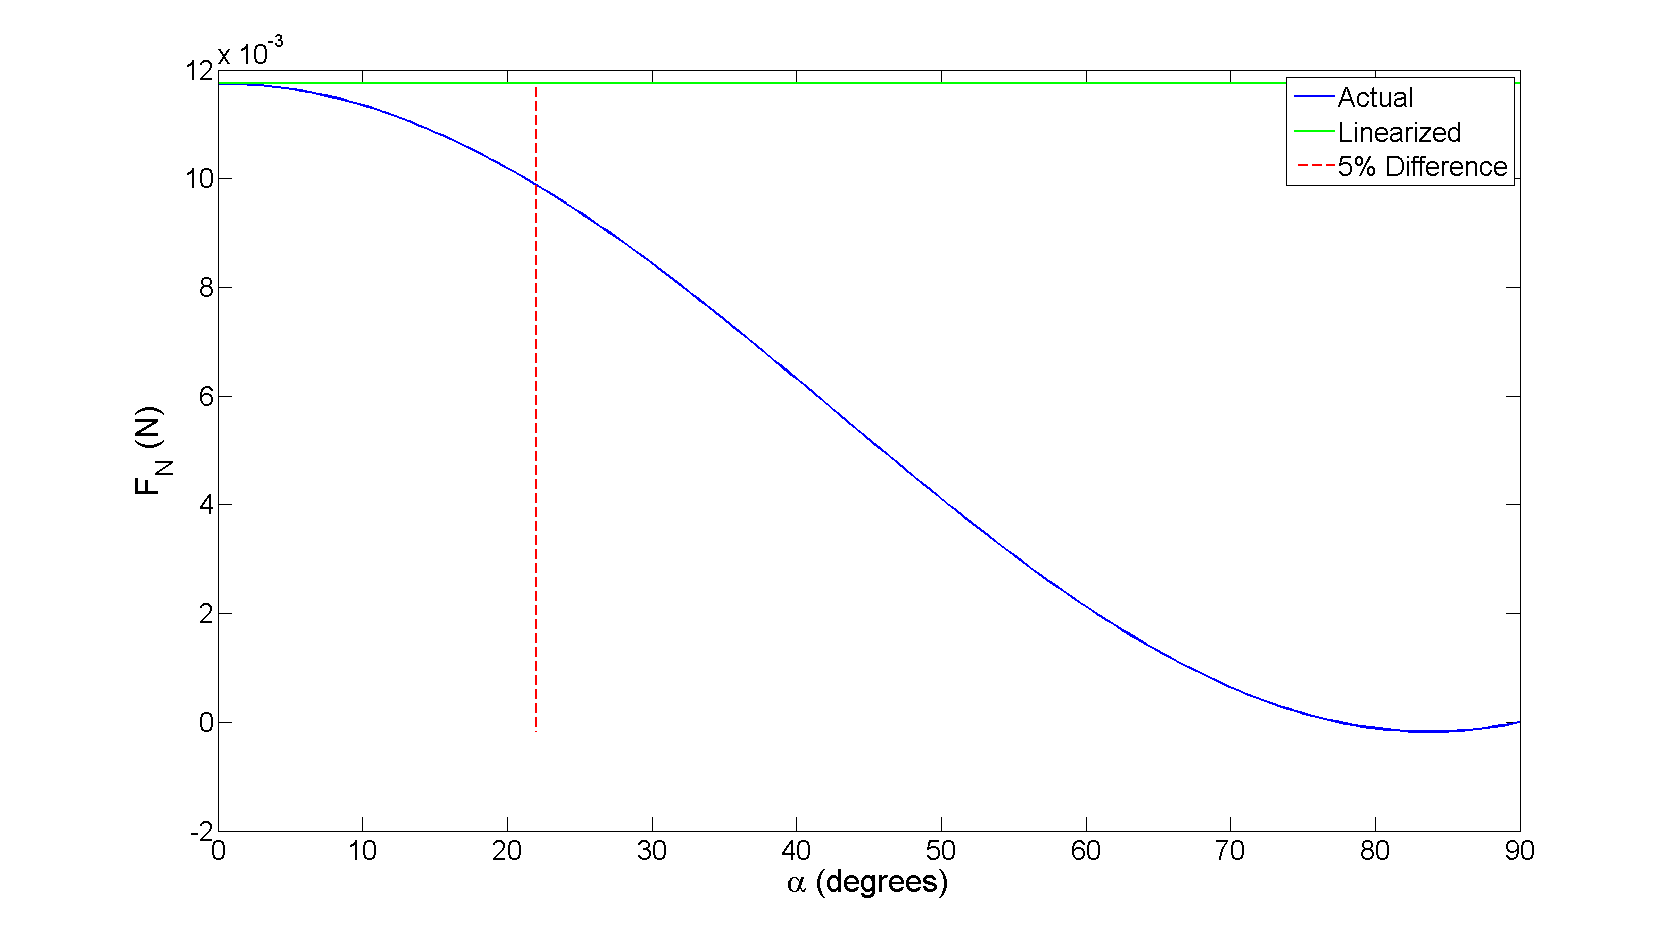
\includegraphics[width = 7.5cm]{FN_Soln.png}
		}
		\caption{Linear solutions of the sail forces vs. sun angle. }
		\label{fig:Force_linearity}
	\end{figure}	

	\vspace{5 mm}

	The controller will be constrained to keep the sun angle less than or equal to 20$^{\circ}$ to keep the system model within the realm of linearity. It will have to dampen the oscillations induced induced by disturbances so that the sail can provide a force in the desired direction. 

	\vspace{5 mm}
	\section{Homework 7}

	The system is found to be controllable since the four-row controllability matrix is full rank.

	\vspace{5 mm}

	For full-state feedback control, pole placement will have to be performed such that the real parts are negative. The gimbal angle cannot exceed $\pm$90$^{\circ}$, which is a physical constraint. To maintain the linearity-about-zero assumption, the sun angle $\alpha$ should not exceed $\pm$20$^{\circ}$. The controller will track the specified sun angle with zero steady-state error.  Due to the slow nature of the changing reference, a nearly-critical damped response will be sufficient.

	\vspace{5 mm}

	The system is found to be observable since the observability matrix is full rank.

	\vspace{5 mm}

	The uncontrolled step response of the system is shown in Figure \ref{fig:StepResp}. The response matches the eigenvalues: two sine waves superimposed on eachother, each corresponding to one of the complex conjugate pairs. Because the eigenvalues have no real part, the motion is undamped.

	\vspace{5 mm}

	\begin{figure}[H]
		\centering
			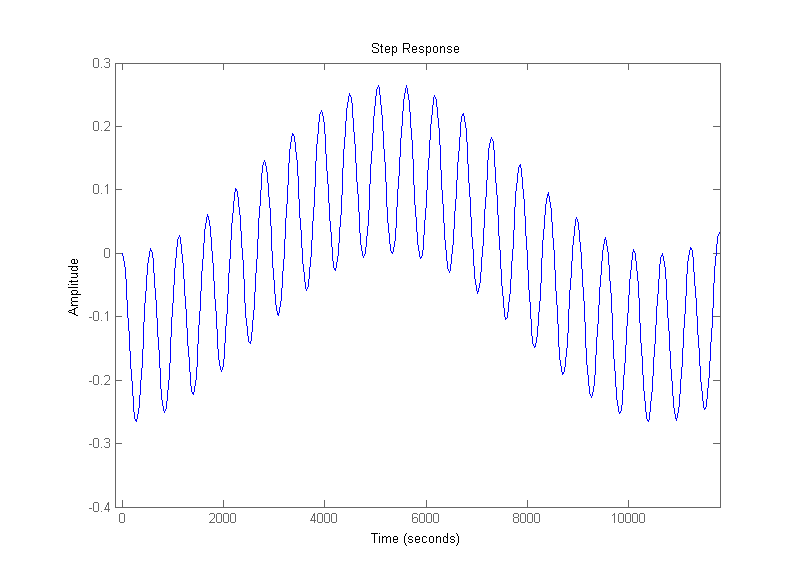
\includegraphics[width = 10cm]{StepResponse.png}
		\caption{Linear solutions of the sail forces vs. sun angle. }
		\label{fig:StepResp}
	\end{figure}	

%    \section{Appendix B}
%This appendix contains all Matlab code used by the authors to analyize their data.
%    
%    \lstset{language=Matlab,%
%    	%basicstyle=\color{red},
%    	breaklines=true,%
%    	morekeywords={matlab2tikz},
%    	keywordstyle=\color{blue},%
%    	morekeywords=[2]{1}, keywordstyle=[2]{\color{black}},
%    	identifierstyle=\color{black},%
%    	stringstyle=\color{mylilas},
%    	commentstyle=\color{mygreen},%
%    	showstringspaces=false,%without this there will be a symbol in the places where there is a space
%    	numbers=left,%
%    	numberstyle={\tiny \color{black}},% size of the numbers
%    	numbersep=9pt, % this defines how far the numbers are from the text
%    	emph=[1]{for,end,break},emphstyle=[1]\color{red}, %some words to emphasise
%    	%emph=[2]{word1,word2}, emphstyle=[2]{style},   
%    }
    
%    \lstinputlisting{ASEN5090_ecef2azelrange.m}
%    \vspace{5mm}
%    
%    \lstinputlisting{ASEN5090_GPSvis.m}
%    \vspace{5mm}
%\lstinputlisting{HW5_rel_err.m}
%\vspace{5mm}
%\lstinputlisting{import_gps_data.m}
%\vspace{5mm}
%\lstinputlisting{datenum8601.m}
%\vspace{5mm}
%\lstinputlisting{lab_err_plots.m}
%\vspace{5mm}
	
\end{document}

% - Release $Name:  $ -
